% Created by tikzDevice version 0.12.6 on 2024-06-11 19:56:29
% !TEX encoding = UTF-8 Unicode
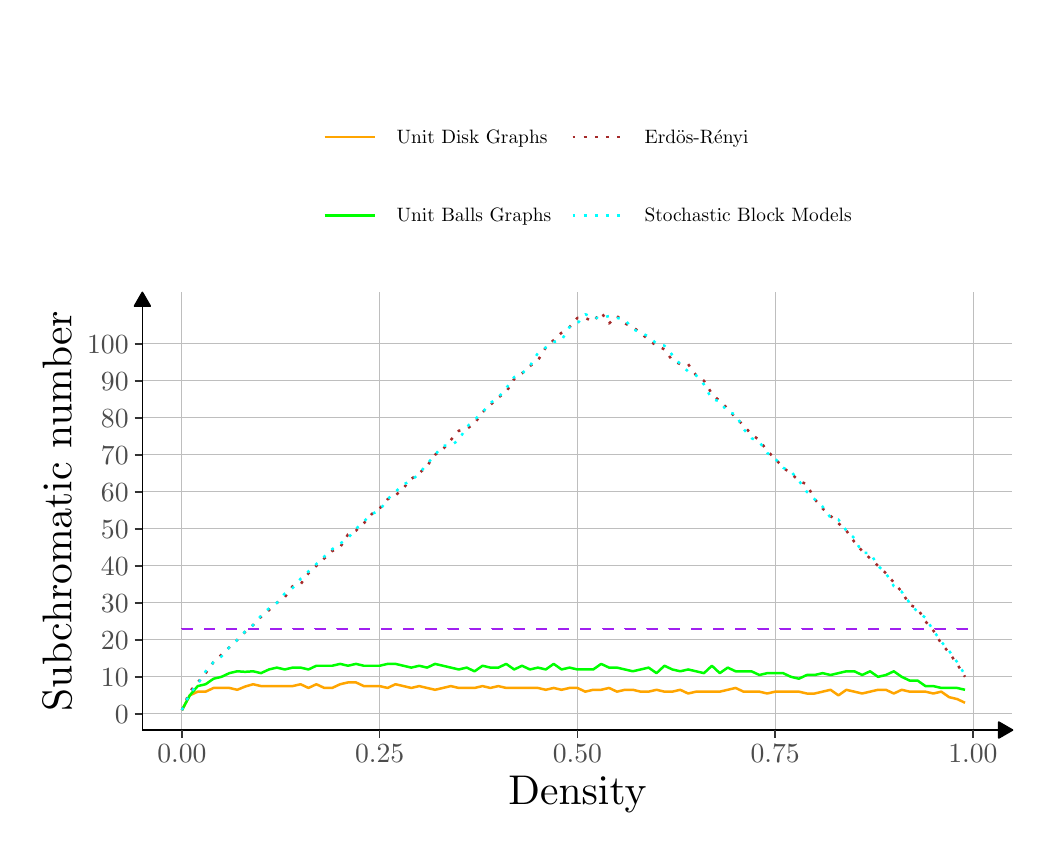
\begin{tikzpicture}[x=1pt,y=1pt]
\definecolor{fillColor}{RGB}{255,255,255}
\path[use as bounding box,fill=fillColor,fill opacity=0.00] (0,0) rectangle (361.35,289.08);
\begin{scope}
\path[clip] (  0.00,  0.00) rectangle (361.35,289.08);
\definecolor{drawColor}{RGB}{255,255,255}
\definecolor{fillColor}{RGB}{255,255,255}

\path[draw=drawColor,line width= 0.6pt,line join=round,line cap=round,fill=fillColor] (  0.00,  0.00) rectangle (361.35,289.08);
\end{scope}
\begin{scope}
\path[clip] ( 41.44, 35.28) rectangle (355.85,193.40);
\definecolor{fillColor}{RGB}{255,255,255}

\path[fill=fillColor] ( 41.44, 35.28) rectangle (355.85,193.40);
\definecolor{drawColor}{RGB}{190,190,190}

\path[draw=drawColor,line width= 0.3pt,line join=round] ( 41.44, 41.13) --
	(355.85, 41.13);

\path[draw=drawColor,line width= 0.3pt,line join=round] ( 41.44, 54.50) --
	(355.85, 54.50);

\path[draw=drawColor,line width= 0.3pt,line join=round] ( 41.44, 67.87) --
	(355.85, 67.87);

\path[draw=drawColor,line width= 0.3pt,line join=round] ( 41.44, 81.24) --
	(355.85, 81.24);

\path[draw=drawColor,line width= 0.3pt,line join=round] ( 41.44, 94.61) --
	(355.85, 94.61);

\path[draw=drawColor,line width= 0.3pt,line join=round] ( 41.44,107.99) --
	(355.85,107.99);

\path[draw=drawColor,line width= 0.3pt,line join=round] ( 41.44,121.36) --
	(355.85,121.36);

\path[draw=drawColor,line width= 0.3pt,line join=round] ( 41.44,134.73) --
	(355.85,134.73);

\path[draw=drawColor,line width= 0.3pt,line join=round] ( 41.44,148.10) --
	(355.85,148.10);

\path[draw=drawColor,line width= 0.3pt,line join=round] ( 41.44,161.47) --
	(355.85,161.47);

\path[draw=drawColor,line width= 0.3pt,line join=round] ( 41.44,174.85) --
	(355.85,174.85);

\path[draw=drawColor,line width= 0.3pt,line join=round] ( 55.73, 35.28) --
	( 55.73,193.40);

\path[draw=drawColor,line width= 0.3pt,line join=round] (127.19, 35.28) --
	(127.19,193.40);

\path[draw=drawColor,line width= 0.3pt,line join=round] (198.65, 35.28) --
	(198.65,193.40);

\path[draw=drawColor,line width= 0.3pt,line join=round] (270.10, 35.28) --
	(270.10,193.40);

\path[draw=drawColor,line width= 0.3pt,line join=round] (341.56, 35.28) --
	(341.56,193.40);
\definecolor{drawColor}{RGB}{255,165,0}

\path[draw=drawColor,line width= 0.9pt,line join=round] ( 55.73, 42.47) --
	( 58.59, 47.81) --
	( 61.45, 49.15) --
	( 64.31, 49.15) --
	( 67.17, 50.49) --
	( 70.03, 50.49) --
	( 72.88, 50.49) --
	( 75.74, 49.82) --
	( 78.60, 51.00) --
	( 81.46, 51.83) --
	( 84.32, 51.16) --
	( 87.18, 51.16) --
	( 90.03, 51.16) --
	( 92.89, 51.16) --
	( 95.75, 51.16) --
	( 98.61, 51.83) --
	(101.47, 50.49) --
	(104.32, 51.83) --
	(107.18, 50.49) --
	(110.04, 50.49) --
	(112.90, 51.83) --
	(115.76, 52.49) --
	(118.62, 52.49) --
	(121.47, 51.16) --
	(124.33, 51.16) --
	(127.19, 51.16) --
	(130.05, 50.49) --
	(132.91, 51.83) --
	(135.77, 51.16) --
	(138.62, 50.49) --
	(141.48, 51.16) --
	(144.34, 50.49) --
	(147.20, 49.82) --
	(150.06, 50.49) --
	(152.91, 51.16) --
	(155.77, 50.49) --
	(158.63, 50.49) --
	(161.49, 50.49) --
	(164.35, 51.16) --
	(167.21, 50.49) --
	(170.06, 51.16) --
	(172.92, 50.49) --
	(175.78, 50.49) --
	(178.64, 50.49) --
	(181.50, 50.49) --
	(184.36, 50.49) --
	(187.21, 49.82) --
	(190.07, 50.49) --
	(192.93, 49.82) --
	(195.79, 50.49) --
	(198.65, 50.49) --
	(201.50, 49.15) --
	(204.36, 49.82) --
	(207.22, 49.82) --
	(210.08, 50.49) --
	(212.94, 49.15) --
	(215.80, 49.82) --
	(218.65, 49.82) --
	(221.51, 49.15) --
	(224.37, 49.15) --
	(227.23, 49.82) --
	(230.09, 49.15) --
	(232.95, 49.15) --
	(235.80, 49.82) --
	(238.66, 48.48) --
	(241.52, 49.15) --
	(244.38, 49.15) --
	(247.24, 49.15) --
	(250.09, 49.15) --
	(252.95, 49.82) --
	(255.81, 50.49) --
	(258.67, 49.15) --
	(261.53, 49.15) --
	(264.39, 49.15) --
	(267.24, 48.48) --
	(270.10, 49.15) --
	(272.96, 49.15) --
	(275.82, 49.15) --
	(278.68, 49.15) --
	(281.54, 48.48) --
	(284.39, 48.48) --
	(287.25, 49.15) --
	(290.11, 49.82) --
	(292.97, 47.81) --
	(295.83, 49.82) --
	(298.69, 49.15) --
	(301.54, 48.48) --
	(304.40, 49.15) --
	(307.26, 49.82) --
	(310.12, 49.82) --
	(312.98, 48.48) --
	(315.83, 49.82) --
	(318.69, 49.15) --
	(321.55, 49.15) --
	(324.41, 49.15) --
	(327.27, 48.48) --
	(330.13, 49.15) --
	(332.98, 47.15) --
	(335.84, 46.48) --
	(338.70, 45.14);
\definecolor{drawColor}{RGB}{0,255,0}

\path[draw=drawColor,line width= 0.9pt,line join=round] ( 55.73, 42.47) --
	( 58.59, 47.81) --
	( 61.45, 51.16) --
	( 64.31, 51.83) --
	( 67.17, 53.83) --
	( 70.03, 54.50) --
	( 72.88, 55.84) --
	( 75.74, 56.51) --
	( 78.60, 56.31) --
	( 81.46, 56.51) --
	( 84.32, 55.84) --
	( 87.18, 57.17) --
	( 90.03, 57.84) --
	( 92.89, 57.17) --
	( 95.75, 57.84) --
	( 98.61, 57.84) --
	(101.47, 57.17) --
	(104.32, 58.51) --
	(107.18, 58.51) --
	(110.04, 58.51) --
	(112.90, 59.18) --
	(115.76, 58.51) --
	(118.62, 59.18) --
	(121.47, 58.51) --
	(124.33, 58.51) --
	(127.19, 58.51) --
	(130.05, 59.18) --
	(132.91, 59.18) --
	(135.77, 58.51) --
	(138.62, 57.84) --
	(141.48, 58.51) --
	(144.34, 57.84) --
	(147.20, 59.18) --
	(150.06, 58.51) --
	(152.91, 57.84) --
	(155.77, 57.17) --
	(158.63, 57.84) --
	(161.49, 56.51) --
	(164.35, 58.51) --
	(167.21, 57.84) --
	(170.06, 57.84) --
	(172.92, 59.18) --
	(175.78, 57.17) --
	(178.64, 58.51) --
	(181.50, 57.17) --
	(184.36, 57.84) --
	(187.21, 57.17) --
	(190.07, 59.18) --
	(192.93, 57.17) --
	(195.79, 57.84) --
	(198.65, 57.17) --
	(201.50, 57.17) --
	(204.36, 57.17) --
	(207.22, 59.18) --
	(210.08, 57.84) --
	(212.94, 57.84) --
	(215.80, 57.17) --
	(218.65, 56.51) --
	(221.51, 57.17) --
	(224.37, 57.84) --
	(227.23, 55.84) --
	(230.09, 58.51) --
	(232.95, 57.17) --
	(235.80, 56.51) --
	(238.66, 57.17) --
	(241.52, 56.51) --
	(244.38, 55.84) --
	(247.24, 58.51) --
	(250.09, 55.84) --
	(252.95, 57.84) --
	(255.81, 56.51) --
	(258.67, 56.51) --
	(261.53, 56.51) --
	(264.39, 55.17) --
	(267.24, 55.84) --
	(270.10, 55.84) --
	(272.96, 55.84) --
	(275.82, 54.50) --
	(278.68, 53.83) --
	(281.54, 55.17) --
	(284.39, 55.17) --
	(287.25, 55.84) --
	(290.11, 55.17) --
	(292.97, 55.84) --
	(295.83, 56.51) --
	(298.69, 56.51) --
	(301.54, 55.17) --
	(304.40, 56.51) --
	(307.26, 54.50) --
	(310.12, 55.17) --
	(312.98, 56.51) --
	(315.83, 54.50) --
	(318.69, 53.16) --
	(321.55, 53.16) --
	(324.41, 51.16) --
	(327.27, 51.16) --
	(330.13, 50.49) --
	(332.98, 50.49) --
	(335.84, 50.49) --
	(338.70, 49.82);
\definecolor{drawColor}{RGB}{165,42,42}

\path[draw=drawColor,line width= 0.9pt,dash pattern=on 1pt off 3pt ,line join=round] ( 55.73, 42.47) --
	( 58.59, 49.15) --
	( 61.45, 52.49) --
	( 64.31, 55.84) --
	( 67.17, 59.85) --
	( 70.03, 62.52) --
	( 72.88, 65.20) --
	( 75.74, 67.87) --
	( 78.60, 70.78) --
	( 81.46, 73.22) --
	( 84.32, 76.17) --
	( 87.18, 78.57) --
	( 90.03, 81.24) --
	( 92.89, 83.25) --
	( 95.75, 87.26) --
	( 98.61, 87.93) --
	(101.47, 91.94) --
	(104.32, 94.61) --
	(107.18, 97.29) --
	(110.04, 99.96) --
	(112.90,101.30) --
	(115.76,105.98) --
	(118.62,107.32) --
	(121.47,109.99) --
	(124.33,113.34) --
	(127.19,115.34) --
	(130.05,118.68) --
	(132.91,120.02) --
	(135.77,122.70) --
	(138.62,126.04) --
	(141.48,128.04) --
	(144.34,130.72) --
	(147.20,134.73) --
	(150.06,136.74) --
	(152.91,140.08) --
	(155.77,143.42) --
	(158.63,144.09) --
	(161.49,146.10) --
	(164.35,150.11) --
	(167.21,152.78) --
	(170.06,155.46) --
	(172.92,157.46) --
	(175.78,162.14) --
	(178.64,164.15) --
	(181.50,166.82) --
	(184.36,168.83) --
	(187.21,173.51) --
	(190.07,176.18) --
	(192.93,178.86) --
	(195.79,180.86) --
	(198.65,184.21) --
	(201.50,184.21) --
	(204.36,182.87) --
	(207.22,186.21) --
	(210.08,182.20) --
	(212.94,184.87) --
	(215.80,182.20) --
	(218.65,180.86) --
	(221.51,178.86) --
	(224.37,176.18) --
	(227.23,174.18) --
	(230.09,172.84) --
	(232.95,168.83) --
	(235.80,167.49) --
	(238.66,167.49) --
	(241.52,163.48) --
	(244.38,161.47) --
	(247.24,156.79) --
	(250.09,154.12) --
	(252.95,151.44) --
	(255.81,148.10) --
	(258.67,145.43) --
	(261.53,142.08) --
	(264.39,140.08) --
	(267.24,136.07) --
	(270.10,133.39) --
	(272.96,130.05) --
	(275.82,128.04) --
	(278.68,125.37) --
	(281.54,124.03) --
	(284.39,118.68) --
	(287.25,115.34) --
	(290.11,112.67) --
	(292.97,109.99) --
	(295.83,107.32) --
	(298.69,103.31) --
	(301.54, 99.96) --
	(304.40, 97.29) --
	(307.26, 94.61) --
	(310.12, 91.94) --
	(312.98, 88.60) --
	(315.83, 85.25) --
	(318.69, 80.57) --
	(321.55, 79.24) --
	(324.41, 74.56) --
	(327.27, 71.21) --
	(330.13, 66.53) --
	(332.98, 63.19) --
	(335.84, 59.18) --
	(338.70, 54.50);
\definecolor{drawColor}{RGB}{0,255,255}

\path[draw=drawColor,line width= 0.9pt,dash pattern=on 1pt off 3pt ,line join=round] ( 55.73, 42.47) --
	( 58.59, 48.48) --
	( 61.45, 51.83) --
	( 64.31, 56.51) --
	( 67.17, 59.85) --
	( 70.03, 61.85) --
	( 72.88, 65.20) --
	( 75.74, 67.87) --
	( 78.60, 70.95) --
	( 81.46, 73.22) --
	( 84.32, 76.58) --
	( 87.18, 79.24) --
	( 90.03, 81.24) --
	( 92.89, 84.59) --
	( 95.75, 86.59) --
	( 98.61, 89.93) --
	(101.47, 92.61) --
	(104.32, 95.28) --
	(107.18, 97.96) --
	(110.04,100.63) --
	(112.90,102.64) --
	(115.76,104.64) --
	(118.62,107.99) --
	(121.47,110.66) --
	(124.33,113.34) --
	(127.19,114.67) --
	(130.05,118.68) --
	(132.91,121.36) --
	(135.77,124.03) --
	(138.62,125.37) --
	(141.48,128.04) --
	(144.34,131.39) --
	(147.20,134.73) --
	(150.06,138.07) --
	(152.91,138.07) --
	(155.77,140.08) --
	(158.63,144.76) --
	(161.49,147.43) --
	(164.35,150.11) --
	(167.21,153.45) --
	(170.06,155.46) --
	(172.92,158.80) --
	(175.78,162.81) --
	(178.64,164.15) --
	(181.50,166.82) --
	(184.36,171.50) --
	(187.21,173.51) --
	(190.07,175.51) --
	(192.93,176.18) --
	(195.79,180.86) --
	(198.65,182.20) --
	(201.50,185.54) --
	(204.36,184.21) --
	(207.22,184.21) --
	(210.08,184.87) --
	(212.94,184.21) --
	(215.80,183.54) --
	(218.65,180.19) --
	(221.51,178.86) --
	(224.37,177.52) --
	(227.23,174.85) --
	(230.09,174.18) --
	(232.95,170.83) --
	(235.80,167.49) --
	(238.66,164.82) --
	(241.52,163.48) --
	(244.38,160.14) --
	(247.24,154.79) --
	(250.09,154.12) --
	(252.95,150.11) --
	(255.81,149.44) --
	(258.67,144.09) --
	(261.53,140.75) --
	(264.39,139.41) --
	(267.24,135.40) --
	(270.10,133.39) --
	(272.96,130.05) --
	(275.82,128.71) --
	(278.68,125.37) --
	(281.54,121.36) --
	(284.39,118.68) --
	(287.25,116.01) --
	(290.11,112.00) --
	(292.97,111.33) --
	(295.83,107.32) --
	(298.69,104.64) --
	(301.54, 99.29) --
	(304.40, 99.29) --
	(307.26, 94.61) --
	(310.12, 91.94) --
	(312.98, 87.26) --
	(315.83, 85.25) --
	(318.69, 81.24) --
	(321.55, 77.90) --
	(324.41, 75.89) --
	(327.27, 71.21) --
	(330.13, 67.20) --
	(332.98, 63.86) --
	(335.84, 59.85) --
	(338.70, 55.17);
\definecolor{drawColor}{RGB}{160,32,240}

\path[draw=drawColor,line width= 0.7pt,dash pattern=on 4pt off 4pt ,line join=round] ( 55.73, 71.88) -- (341.56, 71.88);

\path[draw=drawColor,line width= 0.7pt,dash pattern=on 4pt off 4pt ,line join=round] ( 55.73, 71.88) -- (341.56, 71.88);

\path[draw=drawColor,line width= 0.7pt,dash pattern=on 4pt off 4pt ,line join=round] ( 55.73, 71.88) -- (341.56, 71.88);

\path[draw=drawColor,line width= 0.7pt,dash pattern=on 4pt off 4pt ,line join=round] ( 55.73, 71.88) -- (341.56, 71.88);

\path[draw=drawColor,line width= 0.7pt,dash pattern=on 4pt off 4pt ,line join=round] ( 55.73, 71.88) -- (341.56, 71.88);

\path[draw=drawColor,line width= 0.7pt,dash pattern=on 4pt off 4pt ,line join=round] ( 55.73, 71.88) -- (341.56, 71.88);

\path[draw=drawColor,line width= 0.7pt,dash pattern=on 4pt off 4pt ,line join=round] ( 55.73, 71.88) -- (341.56, 71.88);

\path[draw=drawColor,line width= 0.7pt,dash pattern=on 4pt off 4pt ,line join=round] ( 55.73, 71.88) -- (341.56, 71.88);

\path[draw=drawColor,line width= 0.7pt,dash pattern=on 4pt off 4pt ,line join=round] ( 55.73, 71.88) -- (341.56, 71.88);

\path[draw=drawColor,line width= 0.7pt,dash pattern=on 4pt off 4pt ,line join=round] ( 55.73, 71.88) -- (341.56, 71.88);

\path[draw=drawColor,line width= 0.7pt,dash pattern=on 4pt off 4pt ,line join=round] ( 55.73, 71.88) -- (341.56, 71.88);

\path[draw=drawColor,line width= 0.7pt,dash pattern=on 4pt off 4pt ,line join=round] ( 55.73, 71.88) -- (341.56, 71.88);

\path[draw=drawColor,line width= 0.7pt,dash pattern=on 4pt off 4pt ,line join=round] ( 55.73, 71.88) -- (341.56, 71.88);

\path[draw=drawColor,line width= 0.7pt,dash pattern=on 4pt off 4pt ,line join=round] ( 55.73, 71.88) -- (341.56, 71.88);

\path[draw=drawColor,line width= 0.7pt,dash pattern=on 4pt off 4pt ,line join=round] ( 55.73, 71.88) -- (341.56, 71.88);

\path[draw=drawColor,line width= 0.7pt,dash pattern=on 4pt off 4pt ,line join=round] ( 55.73, 71.88) -- (341.56, 71.88);

\path[draw=drawColor,line width= 0.7pt,dash pattern=on 4pt off 4pt ,line join=round] ( 55.73, 71.88) -- (341.56, 71.88);

\path[draw=drawColor,line width= 0.7pt,dash pattern=on 4pt off 4pt ,line join=round] ( 55.73, 71.88) -- (341.56, 71.88);

\path[draw=drawColor,line width= 0.7pt,dash pattern=on 4pt off 4pt ,line join=round] ( 55.73, 71.88) -- (341.56, 71.88);

\path[draw=drawColor,line width= 0.7pt,dash pattern=on 4pt off 4pt ,line join=round] ( 55.73, 71.88) -- (341.56, 71.88);

\path[draw=drawColor,line width= 0.7pt,dash pattern=on 4pt off 4pt ,line join=round] ( 55.73, 71.88) -- (341.56, 71.88);

\path[draw=drawColor,line width= 0.7pt,dash pattern=on 4pt off 4pt ,line join=round] ( 55.73, 71.88) -- (341.56, 71.88);

\path[draw=drawColor,line width= 0.7pt,dash pattern=on 4pt off 4pt ,line join=round] ( 55.73, 71.88) -- (341.56, 71.88);

\path[draw=drawColor,line width= 0.7pt,dash pattern=on 4pt off 4pt ,line join=round] ( 55.73, 71.88) -- (341.56, 71.88);

\path[draw=drawColor,line width= 0.7pt,dash pattern=on 4pt off 4pt ,line join=round] ( 55.73, 71.88) -- (341.56, 71.88);

\path[draw=drawColor,line width= 0.7pt,dash pattern=on 4pt off 4pt ,line join=round] ( 55.73, 71.88) -- (341.56, 71.88);

\path[draw=drawColor,line width= 0.7pt,dash pattern=on 4pt off 4pt ,line join=round] ( 55.73, 71.88) -- (341.56, 71.88);

\path[draw=drawColor,line width= 0.7pt,dash pattern=on 4pt off 4pt ,line join=round] ( 55.73, 71.88) -- (341.56, 71.88);

\path[draw=drawColor,line width= 0.7pt,dash pattern=on 4pt off 4pt ,line join=round] ( 55.73, 71.88) -- (341.56, 71.88);

\path[draw=drawColor,line width= 0.7pt,dash pattern=on 4pt off 4pt ,line join=round] ( 55.73, 71.88) -- (341.56, 71.88);

\path[draw=drawColor,line width= 0.7pt,dash pattern=on 4pt off 4pt ,line join=round] ( 55.73, 71.88) -- (341.56, 71.88);

\path[draw=drawColor,line width= 0.7pt,dash pattern=on 4pt off 4pt ,line join=round] ( 55.73, 71.88) -- (341.56, 71.88);

\path[draw=drawColor,line width= 0.7pt,dash pattern=on 4pt off 4pt ,line join=round] ( 55.73, 71.88) -- (341.56, 71.88);

\path[draw=drawColor,line width= 0.7pt,dash pattern=on 4pt off 4pt ,line join=round] ( 55.73, 71.88) -- (341.56, 71.88);

\path[draw=drawColor,line width= 0.7pt,dash pattern=on 4pt off 4pt ,line join=round] ( 55.73, 71.88) -- (341.56, 71.88);

\path[draw=drawColor,line width= 0.7pt,dash pattern=on 4pt off 4pt ,line join=round] ( 55.73, 71.88) -- (341.56, 71.88);

\path[draw=drawColor,line width= 0.7pt,dash pattern=on 4pt off 4pt ,line join=round] ( 55.73, 71.88) -- (341.56, 71.88);

\path[draw=drawColor,line width= 0.7pt,dash pattern=on 4pt off 4pt ,line join=round] ( 55.73, 71.88) -- (341.56, 71.88);

\path[draw=drawColor,line width= 0.7pt,dash pattern=on 4pt off 4pt ,line join=round] ( 55.73, 71.88) -- (341.56, 71.88);

\path[draw=drawColor,line width= 0.7pt,dash pattern=on 4pt off 4pt ,line join=round] ( 55.73, 71.88) -- (341.56, 71.88);

\path[draw=drawColor,line width= 0.7pt,dash pattern=on 4pt off 4pt ,line join=round] ( 55.73, 71.88) -- (341.56, 71.88);

\path[draw=drawColor,line width= 0.7pt,dash pattern=on 4pt off 4pt ,line join=round] ( 55.73, 71.88) -- (341.56, 71.88);

\path[draw=drawColor,line width= 0.7pt,dash pattern=on 4pt off 4pt ,line join=round] ( 55.73, 71.88) -- (341.56, 71.88);

\path[draw=drawColor,line width= 0.7pt,dash pattern=on 4pt off 4pt ,line join=round] ( 55.73, 71.88) -- (341.56, 71.88);

\path[draw=drawColor,line width= 0.7pt,dash pattern=on 4pt off 4pt ,line join=round] ( 55.73, 71.88) -- (341.56, 71.88);

\path[draw=drawColor,line width= 0.7pt,dash pattern=on 4pt off 4pt ,line join=round] ( 55.73, 71.88) -- (341.56, 71.88);

\path[draw=drawColor,line width= 0.7pt,dash pattern=on 4pt off 4pt ,line join=round] ( 55.73, 71.88) -- (341.56, 71.88);

\path[draw=drawColor,line width= 0.7pt,dash pattern=on 4pt off 4pt ,line join=round] ( 55.73, 71.88) -- (341.56, 71.88);

\path[draw=drawColor,line width= 0.7pt,dash pattern=on 4pt off 4pt ,line join=round] ( 55.73, 71.88) -- (341.56, 71.88);

\path[draw=drawColor,line width= 0.7pt,dash pattern=on 4pt off 4pt ,line join=round] ( 55.73, 71.88) -- (341.56, 71.88);

\path[draw=drawColor,line width= 0.7pt,dash pattern=on 4pt off 4pt ,line join=round] ( 55.73, 71.88) -- (341.56, 71.88);

\path[draw=drawColor,line width= 0.7pt,dash pattern=on 4pt off 4pt ,line join=round] ( 55.73, 71.88) -- (341.56, 71.88);

\path[draw=drawColor,line width= 0.7pt,dash pattern=on 4pt off 4pt ,line join=round] ( 55.73, 71.88) -- (341.56, 71.88);

\path[draw=drawColor,line width= 0.7pt,dash pattern=on 4pt off 4pt ,line join=round] ( 55.73, 71.88) -- (341.56, 71.88);

\path[draw=drawColor,line width= 0.7pt,dash pattern=on 4pt off 4pt ,line join=round] ( 55.73, 71.88) -- (341.56, 71.88);

\path[draw=drawColor,line width= 0.7pt,dash pattern=on 4pt off 4pt ,line join=round] ( 55.73, 71.88) -- (341.56, 71.88);

\path[draw=drawColor,line width= 0.7pt,dash pattern=on 4pt off 4pt ,line join=round] ( 55.73, 71.88) -- (341.56, 71.88);

\path[draw=drawColor,line width= 0.7pt,dash pattern=on 4pt off 4pt ,line join=round] ( 55.73, 71.88) -- (341.56, 71.88);

\path[draw=drawColor,line width= 0.7pt,dash pattern=on 4pt off 4pt ,line join=round] ( 55.73, 71.88) -- (341.56, 71.88);

\path[draw=drawColor,line width= 0.7pt,dash pattern=on 4pt off 4pt ,line join=round] ( 55.73, 71.88) -- (341.56, 71.88);

\path[draw=drawColor,line width= 0.7pt,dash pattern=on 4pt off 4pt ,line join=round] ( 55.73, 71.88) -- (341.56, 71.88);

\path[draw=drawColor,line width= 0.7pt,dash pattern=on 4pt off 4pt ,line join=round] ( 55.73, 71.88) -- (341.56, 71.88);

\path[draw=drawColor,line width= 0.7pt,dash pattern=on 4pt off 4pt ,line join=round] ( 55.73, 71.88) -- (341.56, 71.88);

\path[draw=drawColor,line width= 0.7pt,dash pattern=on 4pt off 4pt ,line join=round] ( 55.73, 71.88) -- (341.56, 71.88);

\path[draw=drawColor,line width= 0.7pt,dash pattern=on 4pt off 4pt ,line join=round] ( 55.73, 71.88) -- (341.56, 71.88);

\path[draw=drawColor,line width= 0.7pt,dash pattern=on 4pt off 4pt ,line join=round] ( 55.73, 71.88) -- (341.56, 71.88);

\path[draw=drawColor,line width= 0.7pt,dash pattern=on 4pt off 4pt ,line join=round] ( 55.73, 71.88) -- (341.56, 71.88);

\path[draw=drawColor,line width= 0.7pt,dash pattern=on 4pt off 4pt ,line join=round] ( 55.73, 71.88) -- (341.56, 71.88);

\path[draw=drawColor,line width= 0.7pt,dash pattern=on 4pt off 4pt ,line join=round] ( 55.73, 71.88) -- (341.56, 71.88);

\path[draw=drawColor,line width= 0.7pt,dash pattern=on 4pt off 4pt ,line join=round] ( 55.73, 71.88) -- (341.56, 71.88);

\path[draw=drawColor,line width= 0.7pt,dash pattern=on 4pt off 4pt ,line join=round] ( 55.73, 71.88) -- (341.56, 71.88);

\path[draw=drawColor,line width= 0.7pt,dash pattern=on 4pt off 4pt ,line join=round] ( 55.73, 71.88) -- (341.56, 71.88);

\path[draw=drawColor,line width= 0.7pt,dash pattern=on 4pt off 4pt ,line join=round] ( 55.73, 71.88) -- (341.56, 71.88);

\path[draw=drawColor,line width= 0.7pt,dash pattern=on 4pt off 4pt ,line join=round] ( 55.73, 71.88) -- (341.56, 71.88);

\path[draw=drawColor,line width= 0.7pt,dash pattern=on 4pt off 4pt ,line join=round] ( 55.73, 71.88) -- (341.56, 71.88);

\path[draw=drawColor,line width= 0.7pt,dash pattern=on 4pt off 4pt ,line join=round] ( 55.73, 71.88) -- (341.56, 71.88);

\path[draw=drawColor,line width= 0.7pt,dash pattern=on 4pt off 4pt ,line join=round] ( 55.73, 71.88) -- (341.56, 71.88);

\path[draw=drawColor,line width= 0.7pt,dash pattern=on 4pt off 4pt ,line join=round] ( 55.73, 71.88) -- (341.56, 71.88);

\path[draw=drawColor,line width= 0.7pt,dash pattern=on 4pt off 4pt ,line join=round] ( 55.73, 71.88) -- (341.56, 71.88);

\path[draw=drawColor,line width= 0.7pt,dash pattern=on 4pt off 4pt ,line join=round] ( 55.73, 71.88) -- (341.56, 71.88);

\path[draw=drawColor,line width= 0.7pt,dash pattern=on 4pt off 4pt ,line join=round] ( 55.73, 71.88) -- (341.56, 71.88);

\path[draw=drawColor,line width= 0.7pt,dash pattern=on 4pt off 4pt ,line join=round] ( 55.73, 71.88) -- (341.56, 71.88);

\path[draw=drawColor,line width= 0.7pt,dash pattern=on 4pt off 4pt ,line join=round] ( 55.73, 71.88) -- (341.56, 71.88);

\path[draw=drawColor,line width= 0.7pt,dash pattern=on 4pt off 4pt ,line join=round] ( 55.73, 71.88) -- (341.56, 71.88);

\path[draw=drawColor,line width= 0.7pt,dash pattern=on 4pt off 4pt ,line join=round] ( 55.73, 71.88) -- (341.56, 71.88);

\path[draw=drawColor,line width= 0.7pt,dash pattern=on 4pt off 4pt ,line join=round] ( 55.73, 71.88) -- (341.56, 71.88);

\path[draw=drawColor,line width= 0.7pt,dash pattern=on 4pt off 4pt ,line join=round] ( 55.73, 71.88) -- (341.56, 71.88);

\path[draw=drawColor,line width= 0.7pt,dash pattern=on 4pt off 4pt ,line join=round] ( 55.73, 71.88) -- (341.56, 71.88);

\path[draw=drawColor,line width= 0.7pt,dash pattern=on 4pt off 4pt ,line join=round] ( 55.73, 71.88) -- (341.56, 71.88);

\path[draw=drawColor,line width= 0.7pt,dash pattern=on 4pt off 4pt ,line join=round] ( 55.73, 71.88) -- (341.56, 71.88);

\path[draw=drawColor,line width= 0.7pt,dash pattern=on 4pt off 4pt ,line join=round] ( 55.73, 71.88) -- (341.56, 71.88);

\path[draw=drawColor,line width= 0.7pt,dash pattern=on 4pt off 4pt ,line join=round] ( 55.73, 71.88) -- (341.56, 71.88);

\path[draw=drawColor,line width= 0.7pt,dash pattern=on 4pt off 4pt ,line join=round] ( 55.73, 71.88) -- (341.56, 71.88);

\path[draw=drawColor,line width= 0.7pt,dash pattern=on 4pt off 4pt ,line join=round] ( 55.73, 71.88) -- (341.56, 71.88);

\path[draw=drawColor,line width= 0.7pt,dash pattern=on 4pt off 4pt ,line join=round] ( 55.73, 71.88) -- (341.56, 71.88);

\path[draw=drawColor,line width= 0.7pt,dash pattern=on 4pt off 4pt ,line join=round] ( 55.73, 71.88) -- (341.56, 71.88);

\path[draw=drawColor,line width= 0.7pt,dash pattern=on 4pt off 4pt ,line join=round] ( 55.73, 71.88) -- (341.56, 71.88);

\path[draw=drawColor,line width= 0.7pt,dash pattern=on 4pt off 4pt ,line join=round] ( 55.73, 71.88) -- (341.56, 71.88);

\path[draw=drawColor,line width= 0.7pt,dash pattern=on 4pt off 4pt ,line join=round] ( 55.73, 71.88) -- (341.56, 71.88);

\path[draw=drawColor,line width= 0.7pt,dash pattern=on 4pt off 4pt ,line join=round] ( 55.73, 71.88) -- (341.56, 71.88);
\end{scope}
\begin{scope}
\path[clip] (  0.00,  0.00) rectangle (361.35,289.08);
\definecolor{drawColor}{RGB}{0,0,0}

\path[draw=drawColor,line width= 0.6pt,line join=round] ( 41.44, 35.28) --
	( 41.44,193.40);
\definecolor{fillColor}{RGB}{0,0,0}

\path[draw=drawColor,line width= 0.6pt,line join=round,fill=fillColor] ( 44.29,188.47) --
	( 41.44,193.40) --
	( 38.60,188.47) --
	cycle;
\end{scope}
\begin{scope}
\path[clip] (  0.00,  0.00) rectangle (361.35,289.08);
\definecolor{drawColor}{gray}{0.30}

\node[text=drawColor,anchor=base east,inner sep=0pt, outer sep=0pt, scale=  1.00] at ( 36.49, 37.68) {0};

\node[text=drawColor,anchor=base east,inner sep=0pt, outer sep=0pt, scale=  1.00] at ( 36.49, 51.06) {10};

\node[text=drawColor,anchor=base east,inner sep=0pt, outer sep=0pt, scale=  1.00] at ( 36.49, 64.43) {20};

\node[text=drawColor,anchor=base east,inner sep=0pt, outer sep=0pt, scale=  1.00] at ( 36.49, 77.80) {30};

\node[text=drawColor,anchor=base east,inner sep=0pt, outer sep=0pt, scale=  1.00] at ( 36.49, 91.17) {40};

\node[text=drawColor,anchor=base east,inner sep=0pt, outer sep=0pt, scale=  1.00] at ( 36.49,104.54) {50};

\node[text=drawColor,anchor=base east,inner sep=0pt, outer sep=0pt, scale=  1.00] at ( 36.49,117.91) {60};

\node[text=drawColor,anchor=base east,inner sep=0pt, outer sep=0pt, scale=  1.00] at ( 36.49,131.29) {70};

\node[text=drawColor,anchor=base east,inner sep=0pt, outer sep=0pt, scale=  1.00] at ( 36.49,144.66) {80};

\node[text=drawColor,anchor=base east,inner sep=0pt, outer sep=0pt, scale=  1.00] at ( 36.49,158.03) {90};

\node[text=drawColor,anchor=base east,inner sep=0pt, outer sep=0pt, scale=  1.00] at ( 36.49,171.40) {100};
\end{scope}
\begin{scope}
\path[clip] (  0.00,  0.00) rectangle (361.35,289.08);
\definecolor{drawColor}{gray}{0.20}

\path[draw=drawColor,line width= 0.6pt,line join=round] ( 38.69, 41.13) --
	( 41.44, 41.13);

\path[draw=drawColor,line width= 0.6pt,line join=round] ( 38.69, 54.50) --
	( 41.44, 54.50);

\path[draw=drawColor,line width= 0.6pt,line join=round] ( 38.69, 67.87) --
	( 41.44, 67.87);

\path[draw=drawColor,line width= 0.6pt,line join=round] ( 38.69, 81.24) --
	( 41.44, 81.24);

\path[draw=drawColor,line width= 0.6pt,line join=round] ( 38.69, 94.61) --
	( 41.44, 94.61);

\path[draw=drawColor,line width= 0.6pt,line join=round] ( 38.69,107.99) --
	( 41.44,107.99);

\path[draw=drawColor,line width= 0.6pt,line join=round] ( 38.69,121.36) --
	( 41.44,121.36);

\path[draw=drawColor,line width= 0.6pt,line join=round] ( 38.69,134.73) --
	( 41.44,134.73);

\path[draw=drawColor,line width= 0.6pt,line join=round] ( 38.69,148.10) --
	( 41.44,148.10);

\path[draw=drawColor,line width= 0.6pt,line join=round] ( 38.69,161.47) --
	( 41.44,161.47);

\path[draw=drawColor,line width= 0.6pt,line join=round] ( 38.69,174.85) --
	( 41.44,174.85);
\end{scope}
\begin{scope}
\path[clip] (  0.00,  0.00) rectangle (361.35,289.08);
\definecolor{drawColor}{RGB}{0,0,0}

\path[draw=drawColor,line width= 0.6pt,line join=round] ( 41.44, 35.28) --
	(355.85, 35.28);
\definecolor{fillColor}{RGB}{0,0,0}

\path[draw=drawColor,line width= 0.6pt,line join=round,fill=fillColor] (350.92, 32.43) --
	(355.85, 35.28) --
	(350.92, 38.12) --
	cycle;
\end{scope}
\begin{scope}
\path[clip] (  0.00,  0.00) rectangle (361.35,289.08);
\definecolor{drawColor}{gray}{0.20}

\path[draw=drawColor,line width= 0.6pt,line join=round] ( 55.73, 32.53) --
	( 55.73, 35.28);

\path[draw=drawColor,line width= 0.6pt,line join=round] (127.19, 32.53) --
	(127.19, 35.28);

\path[draw=drawColor,line width= 0.6pt,line join=round] (198.65, 32.53) --
	(198.65, 35.28);

\path[draw=drawColor,line width= 0.6pt,line join=round] (270.10, 32.53) --
	(270.10, 35.28);

\path[draw=drawColor,line width= 0.6pt,line join=round] (341.56, 32.53) --
	(341.56, 35.28);
\end{scope}
\begin{scope}
\path[clip] (  0.00,  0.00) rectangle (361.35,289.08);
\definecolor{drawColor}{gray}{0.30}

\node[text=drawColor,anchor=base,inner sep=0pt, outer sep=0pt, scale=  1.00] at ( 55.73, 23.44) {0.00};

\node[text=drawColor,anchor=base,inner sep=0pt, outer sep=0pt, scale=  1.00] at (127.19, 23.44) {0.25};

\node[text=drawColor,anchor=base,inner sep=0pt, outer sep=0pt, scale=  1.00] at (198.65, 23.44) {0.50};

\node[text=drawColor,anchor=base,inner sep=0pt, outer sep=0pt, scale=  1.00] at (270.10, 23.44) {0.75};

\node[text=drawColor,anchor=base,inner sep=0pt, outer sep=0pt, scale=  1.00] at (341.56, 23.44) {1.00};
\end{scope}
\begin{scope}
\path[clip] (  0.00,  0.00) rectangle (361.35,289.08);
\definecolor{drawColor}{RGB}{0,0,0}

\node[text=drawColor,anchor=base,inner sep=0pt, outer sep=0pt, scale=  1.50] at (198.65,  8.42) {Density};
\end{scope}
\begin{scope}
\path[clip] (  0.00,  0.00) rectangle (361.35,289.08);
\definecolor{drawColor}{RGB}{0,0,0}

\node[text=drawColor,rotate= 90.00,anchor=base,inner sep=0pt, outer sep=0pt, scale=  1.50] at ( 15.83,114.34) {Subchromatic number};
\end{scope}
\begin{scope}
\path[clip] (  0.00,  0.00) rectangle (361.35,289.08);
\definecolor{fillColor}{RGB}{255,255,255}

\path[fill=fillColor] ( 94.05,204.40) rectangle (303.24,266.42);
\end{scope}
\begin{scope}
\path[clip] (  0.00,  0.00) rectangle (361.35,289.08);
\definecolor{fillColor}{RGB}{255,255,255}

\path[fill=fillColor] (105.05,238.16) rectangle (127.81,260.92);
\end{scope}
\begin{scope}
\path[clip] (  0.00,  0.00) rectangle (361.35,289.08);
\definecolor{drawColor}{RGB}{255,165,0}

\path[draw=drawColor,line width= 0.9pt,line join=round] (107.33,249.54) -- (125.54,249.54);
\end{scope}
\begin{scope}
\path[clip] (  0.00,  0.00) rectangle (361.35,289.08);
\definecolor{fillColor}{RGB}{255,255,255}

\path[fill=fillColor] (105.05,209.90) rectangle (127.81,232.66);
\end{scope}
\begin{scope}
\path[clip] (  0.00,  0.00) rectangle (361.35,289.08);
\definecolor{drawColor}{RGB}{0,255,0}

\path[draw=drawColor,line width= 0.9pt,line join=round] (107.33,221.28) -- (125.54,221.28);
\end{scope}
\begin{scope}
\path[clip] (  0.00,  0.00) rectangle (361.35,289.08);
\definecolor{fillColor}{RGB}{255,255,255}

\path[fill=fillColor] (194.66,238.16) rectangle (217.42,260.92);
\end{scope}
\begin{scope}
\path[clip] (  0.00,  0.00) rectangle (361.35,289.08);
\definecolor{drawColor}{RGB}{165,42,42}

\path[draw=drawColor,line width= 0.9pt,dash pattern=on 1pt off 3pt ,line join=round] (196.93,249.54) -- (215.14,249.54);
\end{scope}
\begin{scope}
\path[clip] (  0.00,  0.00) rectangle (361.35,289.08);
\definecolor{fillColor}{RGB}{255,255,255}

\path[fill=fillColor] (194.66,209.90) rectangle (217.42,232.66);
\end{scope}
\begin{scope}
\path[clip] (  0.00,  0.00) rectangle (361.35,289.08);
\definecolor{drawColor}{RGB}{0,255,255}

\path[draw=drawColor,line width= 0.9pt,dash pattern=on 1pt off 3pt ,line join=round] (196.93,221.28) -- (215.14,221.28);
\end{scope}
\begin{scope}
\path[clip] (  0.00,  0.00) rectangle (361.35,289.08);
\definecolor{drawColor}{RGB}{0,0,0}

\node[text=drawColor,anchor=base west,inner sep=0pt, outer sep=0pt, scale=  0.70] at (133.31,247.13) {Unit Disk Graphs};
\end{scope}
\begin{scope}
\path[clip] (  0.00,  0.00) rectangle (361.35,289.08);
\definecolor{drawColor}{RGB}{0,0,0}

\node[text=drawColor,anchor=base west,inner sep=0pt, outer sep=0pt, scale=  0.70] at (133.31,218.87) {Unit Balls Graphs};
\end{scope}
\begin{scope}
\path[clip] (  0.00,  0.00) rectangle (361.35,289.08);
\definecolor{drawColor}{RGB}{0,0,0}

\node[text=drawColor,anchor=base west,inner sep=0pt, outer sep=0pt, scale=  0.70] at (222.92,247.13) {Erdös-Rényi};
\end{scope}
\begin{scope}
\path[clip] (  0.00,  0.00) rectangle (361.35,289.08);
\definecolor{drawColor}{RGB}{0,0,0}

\node[text=drawColor,anchor=base west,inner sep=0pt, outer sep=0pt, scale=  0.70] at (222.92,218.87) {Stochastic Block Models};
\end{scope}
\end{tikzpicture}
